\documentclass[12pt]{amsart}
\usepackage{amsaddr}
\usepackage[draft]{../marktext} 
%% Remove draft for real article, put twocolumn for two columns
\usepackage[draft]{../svmacro}
\usepackage[utf8]{inputenc}
\usepackage[style=alphabetic, backend=biber]{biblatex}
\addbibresource{bibliography.bib}

%% commentary bubble
\newcommand{\SV}[2][]{\sidenote[colback=green!10]{\textbf{SV\xspace #1:} #2}}

%% Title 
\title{ Worksheet 11}
\author{MATH 101}
\address{Fulbright University, Ho Chi Minh City, Vietnam}

%\author{Co-author}
%\address{  }
%\email {  }
%
\date{\today}

\begin{document}

\maketitle

\section*{Approximations}

\begin{question}
	From the video of 3Blue1Brown, summarize what is Taylor series?
	A reference for Taylor series is here: \url{https://tutorial.math.lamar.edu/classes/calcii/taylorseries.aspx}

	Another reference to learn about why infinite series is fun by
	one of the finest mathematicians in this generation, Charles Fefferman (Princeton University):
	\url{https://www.youtube.com/watch?v=Jwtn5_d2YCs}
\end{question}

\newpage

\begin{question}
	Find the Taylor series for the following functions:
	\begin{enumerate}
		\item $\sin(x)$
		      \vspace{5cm}
		\item $e^x$
		      \vspace{5cm}
		\item $\ln (1 + x) $
		      \vspace{5cm}
	\end{enumerate}
\end{question}



\newpage






\section*{Optimization}

The meaning of second derivative is that it tells us about the concavity of the graph of a function.


\begin{center}
	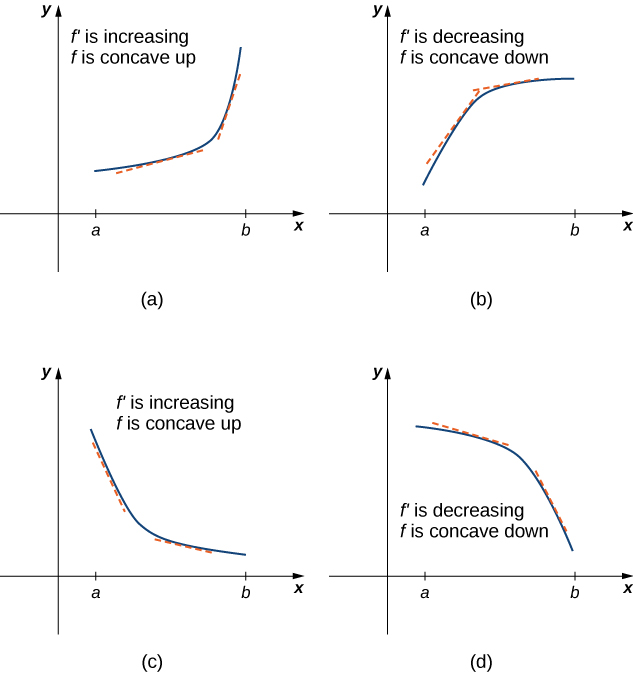
\includegraphics{fig3.jpeg}
\end{center}



\begin{definition}
	Let \( f \) be a function defined over an interval \( I \) and let \( c \in I \).
	We say \( f \) has an absolute maximum on \( I \) at \( c \) if \( f(c) \geq f(x) \) for all \( x \in I \).
	We say \( f \) has an absolute minimum on \( I \) at \( c \) if \( f(c) \leq f(x) \) for all \( x \in I \).
	If \( f \) has an absolute maximum on \( I \) at \( c \) or an absolute minimum on \( I \) at \( c \), we say \( f \) has an absolute extremum on \( I \) at \( c \).
\end{definition}


\begin{theorem}
	If \( f \) is a continuous function over the closed, bounded interval \([a, b]\),
	then there is a point in \([a, b]\) at which \( f \) has an absolute maximum over \([a, b]\),
	and there is a point in \([a, b]\) at which \( f \) has an absolute minimum over \([a, b]\).
\end{theorem}



\end{document}
